\begin{homeworkProblem}

\textbf{Standard Normal Distribution:} generate samples from the standard normal distribution

(a) Implement a Metropolis-Hastings algorithm.

(b) Implement a Hamiltonian Monte Carlo algorithm.

(c) Implement with the Box-Muller Method.

(d) Compare the above three algorithms with corresponding pros and cons.

\solution

(a) Let $X\sim \N(0,1)$, and $Y=|X|$. So $X\in (-\infty,+\infty)$, $Y\in (0,+\infty)$. We can get the PDF of the stationary distribution:
$$\pi_i=\dfrac{2}{\sqrt{2\pi}}e^{-\frac{1}{2}i^2},i>0$$
And we can choose the proposal distribution to be $\Expo(1)$, which means that the one-step transition probability density from state $x$ to $y$ is $f_{x,y}=f_{X_{n+1}|X_n}(y|x)=e^{-y},y>0$, thus we can get that the acceptance rate:
$$a_{i,j}=\min\left(\dfrac{\pi_jf_{j,i}}{\pi_if_{i,j}},1\right)=\min\left(e^{-\frac{1}{2}j^2+j+\frac{1}{2}i^2-i},1\right)$$
Then we can do the Discrete time continuous state Metropolis-Hastings algorithm to sample the distribution of $Y$. \\
To sample on $X\sim \N(0,1)$, since $Y=|X|$, so we can generate $U\sim\Unif(0,1)$, and let $X=\begin{cases}
    Y, & U\leq \frac{1}{2} \\
    -Y, & U>\frac{1}{2}
\end{cases}$. \\
Thus the $\N(0,1)$ is sampled with Metropolis-Hastings algorithm in 1000000 samples, and the burn in is set to be 10000 samples. The result is as follows:
\begin{figure}[h]
    \centering
    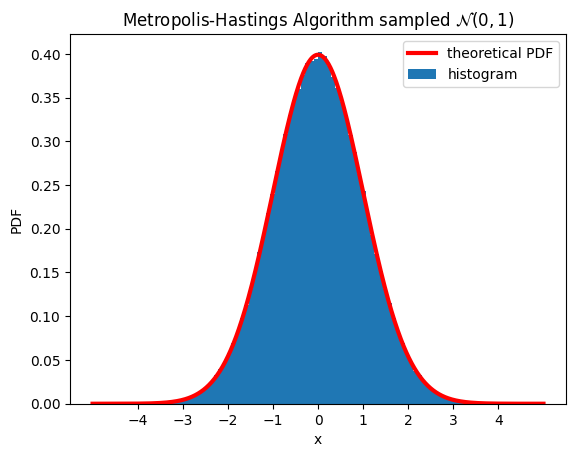
\includegraphics[width=0.4\textwidth]{./figure/p4/MH.png}
\end{figure}

(b) Since $\pi_x$ is a the stationary distribution $\N(0,1)$, and we can ignore the constant form, so the potential energy is
$$U(x)=-\log(\pi_x)=\dfrac{1}{2}x^2 + \dfrac{1}{2}\log(2\pi) \stackrel{\text{ignore const}}{\Rightarrow} U(x)=\dfrac{1}{2}x^2$$
And let the mass be 1. There exists a problem that we need to sample is $\N(0,1)$, so we cannot $\N(0,1)$ as the distribution for Kinetic energy. So we can set the Kinetic energy to be a Student's t-distribution with parameter $\nu=1$, thus then the Kinetic energy is
$$V(\omega)\stackrel{\text{ignore constant}}{=}\dfrac{\nu+1}{2}\log\left(1+\dfrac{\omega^2}{\nu}\right) \qquad\text{where } \omega\sim\text{Student-t}(\nu=1)$$
Thus the Hamiltonian energy is
$$H(x,\omega)=U(x)+V(\omega)=\dfrac{1}{2}x^2+\dfrac{\nu+1}{2}\log\left(1+\dfrac{\omega^2}{\nu}\right)$$
Initially, set $x_0=0, \omega_0\sim\N(0,1)$, apply the Leapfrog method to sample:
\begin{align*}
\omega_{t+\frac{\delta}{2}} &= \omega_t - \frac{\delta}{2}\cdot \dfrac{\dU(x_t)}{\dx_t} = \omega_t - \frac{\delta}{2}\cdot x_t \\
x_{t+\delta} &= x_t + \delta \cdot \dfrac{\dV(\omega_{t+\frac{\delta}{2}})}{\domega_{t+\frac{\delta}{2}}} = x_t + \delta\cdot \dfrac{\nu + 1}{\nu} * \dfrac{\omega_{t+\frac{\delta}{2}}}{1 + \frac{\omega_{t+\frac{\delta}{2}}^2}{\nu}} \\
\omega_{t+\delta} &= \omega_{t+\frac{\delta}{2}} - \frac{\delta}{2}\cdot \dfrac{\dU(x_{t+\delta})}{\dx_{t+\delta}} = \omega_{t+\frac{\delta}{2}} - \frac{\delta}{2}\cdot x_{t+\delta}
\end{align*}
After Leapfrog $L$ steps, we can get the state $(x_L, \omega_L)$. And set $(x_L, -\omega_L)$ to be the proposal distribution. And the accept rate for the Hamiltonian Monte Carlo algorithm is
$$a_{(x_0,\omega_0),(x_L,-\omega_L)}=\min\left(\dfrac{\exp\left(-H(x_L,-\omega_L)\right)}{\exp\left(-H(x_0,\omega_0)\right)}, 1\right)=\min\left(\dfrac{\exp\left(-U(x_L)-V(-\omega_L)\right)}{\exp\left(-U(x_0)-V(\omega_0)\right)}, 1\right)$$
We step the stepsize to be $\delta=0.3, L=15$, and the sample trajectory of one step's LeapFrog and sample results are as follows:
\begin{figure}[h]
    \centering
    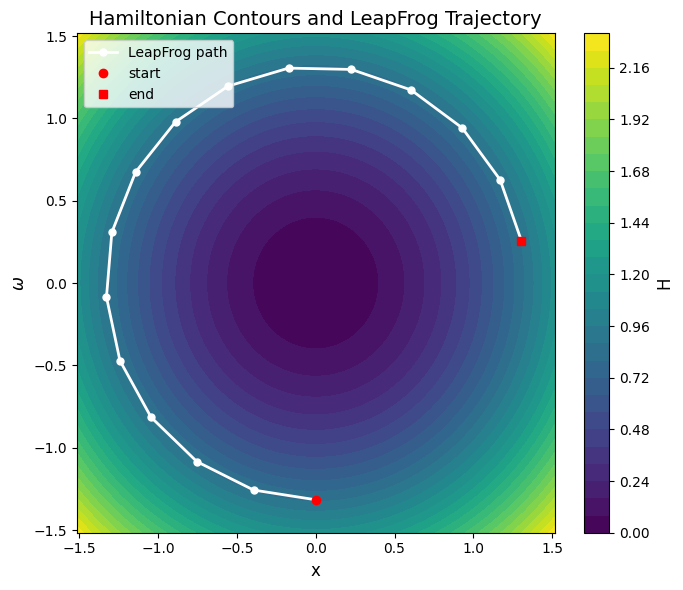
\includegraphics[width=0.5\textwidth]{./figure/p4/trajectory.png}
    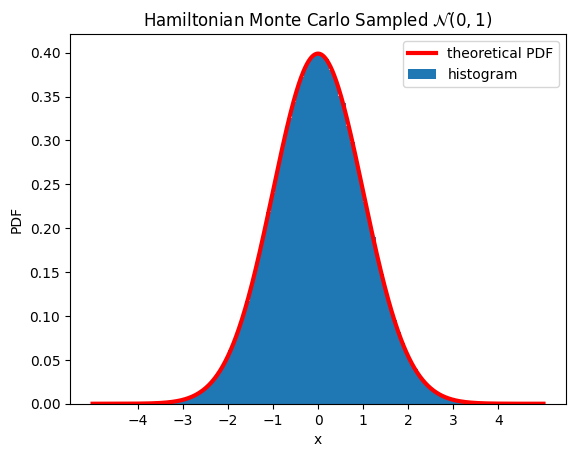
\includegraphics[width=0.5\textwidth]{./figure/p4/Hamiltonian.png}
\end{figure}

(c) Let $U\sim \Unif(0,2\pi)$, so $f_U(u)=\dfrac{1}{2\pi},u\in [0,2\pi]$, which is easy to sample. Let $T\sim \Expo(1)$, so $f_T(t)=e^{-t}, t\in (0,+\infty)$. To sample on $T$, we can use the Universality of Uniform: the Exponential distribution has CDF
$$F_T(t) = 1 - e^{-t}, \forall t > 0$$
So the inverse funciton of its CDF is $ F^{-1}_T(x) = -\ln(1-x)$. So let $U_2\sim \Unif(0,1)$, then
$$T = F^{-1}(U_2)=-\ln(1-U_2)$$
Let $X=\sqrt{2T}\cos(U), Y=\sqrt{2T}\sin(U)$, from Box-Muller method, we can get that $X,Y$ are i.i.d. $\N(0,1)$. The sampled results are as follows:
\begin{figure}[h]
    \centering
    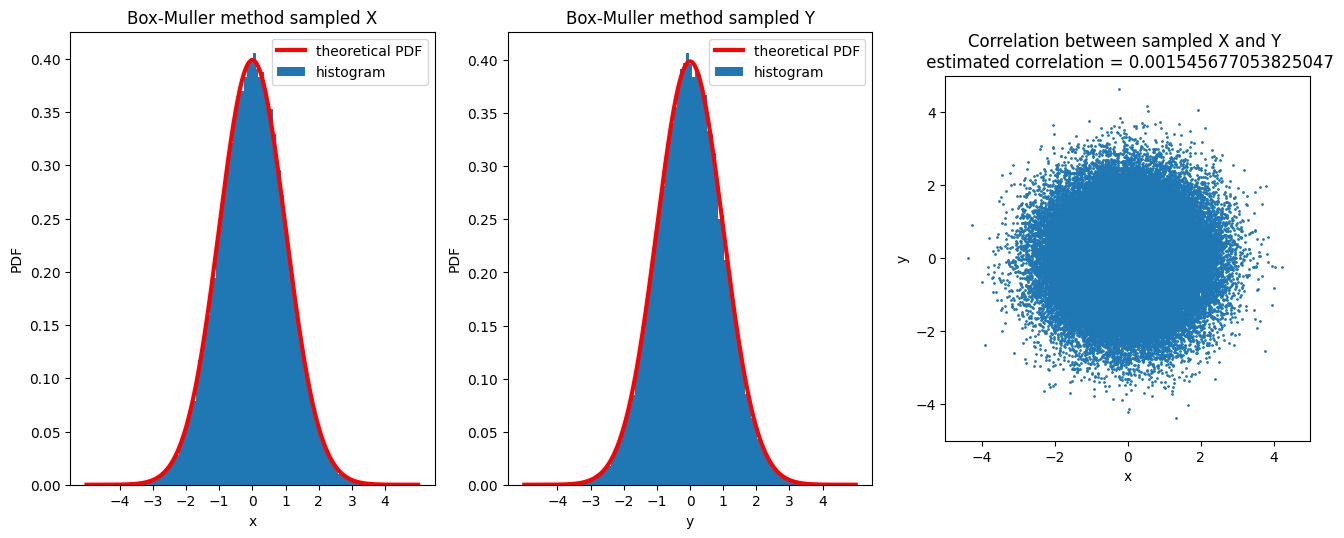
\includegraphics[width=0.8\textwidth]{./figure/p4/box_muller.png}
\end{figure}

(d) 1. Metropolis-Hastings Algorithm: \\
Advantages: It is highly general-purpose, could applicable to a wide variety of distributions, and it does not require the normalization constant of the target distribution. \\
Disadvantages: Samples are often requires select a suitable distribution, and requires steps to burn up.

2. Hamiltonian Monte Carlo Algorithm: \\
Advantages: Due to the conservation of energy, the acceptance rate should be $1$. But there exists numerical error, however quite close to $1$, which means it has quite high acceptance rate. The samples are efficient, especially in high-dimensional problems. \\
Disadvantages: Requires computation of gradients, increasing implementation complexity. Sensitive to parameters: step size $\delta$ and number of steps for LeapFrog $L$.

3. Box-Muller Method: \\
Advantages: Direct and simple method to generate independent standard normal samples, which is easy to implement. \\
Disadvantages: It would sample the normal distribution only.

\end{homeworkProblem}

\newpage